\section{问题二：异构无人机多点多架次运输调度}
\label{sec:q2}

\subsection{问题分析与模型建立}

问题二在问题一的基础上新增了三类强耦合：\textbf{①}架次可访问多个服务区，导致载荷沿航段\textbf{逐段递减}；\textbf{②}三种机型异构，容量、速度与能耗各不相同，机型本身成为决策变量；\textbf{③}共享电池与两阶段充电周转使\textbf{资源可用性}成为真正的瓶颈。需要联合确定的决策变量构成一个六元组：货箱组批、服务区访问顺序、运输机型、具体执行的实体无人机、共享电池分配、各架次开始时刻。

\textbf{（1）多点串飞的前缀容量约束。}设架次 $p$ 的访问顺序为 $(S_a,S_b,\dots)$，则当无人机飞到第 $m$ 站时，机上仍载有第 $m$ 站及之后各站的货物。因此容量约束必须对\textbf{每一个前缀}成立：
\begin{equation}
	\label{eq:21}
	\forall m:\quad\sum_{k\ge m}m_{k}\le Q_{g},\qquad \sum_{k\ge m}v_{k}\le V_{g}
\end{equation}
式中的求和下标含义是“从第 $m$ 站起仍留在机上的货”，而非全架次总量。

\textbf{（2）逐段能耗。}由于能耗关于距离\textbf{非线性}（经由 $L_{g}(q)$）、且载荷逐段递减，架次能耗必须\textbf{逐段累加}，不能把多段距离相加当作一段计算：
\begin{equation}
	\label{eq:22}
	E_{p}^{T}=\sum_{m}E_{g}\big(seg_{m},\,q_{m}\big)\le(1-\rho_{g})\cdot E_{g}^{use}
\end{equation}
其中 $q_{m}$ 为第 $m$ 段上的实际机上载荷，最后一段（返程）取 0。

\textbf{（3）架次总作业时间。}交接时间必须\textbf{按站累加}，即每站各计一次基础交接时间加该站箱数的增量时间：
\begin{equation}
	\label{eq:23}
	\begin{aligned}
		t_{p}={}&t_{prep}+n_{box}\cdot t_{load}+\sum_{m}t_{g}(seg_{m})\\
		      &+\sum_{s\in stops}\big(t_{h0}+k_{s}\cdot t_{h1}\big)
	\end{aligned}
\end{equation}
这里 $k_{s}$ 为在第 $s$ 站投送的箱数。若误写成“（基础交接 $+$ 每箱时间 $\times$ 总箱数）$\times$ 站数”，会把基础交接重复乘上总箱数，严重高估时间窗。

\textbf{（4）时限约束。}两类时限需严格区分：\textbf{首批保障箱}须满足首批截止时间 $d_{b}^{fb}$，\textbf{全部货箱}须衡量是否满足期望送达时间 $d_{b}^{exp}$：
\begin{equation}
	\label{eq:24}
	\begin{aligned}
		t_{b}^{deliver}&\le d_{b}^{fb}\quad(\text{仅首批保障箱}),\\
		t_{b}^{deliver}&\le d_{b}^{exp}\quad(\text{全部货箱})
	\end{aligned}
\end{equation}

多点多架次调度在结构上属于多趟车辆路径问题（multi-trip VRP）的无人机变体\cite{choi2019multitrip,luo2017twoechelon,yang2025lodbo}。

\textbf{（5）多目标。}本文采用\textbf{字典序}目标，依次为：配送及时性惩罚 $>$ 架次数 $>$ 运输能耗。多目标应急调度亦可采用 NSGA-II 等进化算法求取 Pareto 前沿\cite{deb2002nsga2}，本文因其解集规模小、且时限优先级明确而选择字典序处理。其依据是应急场景下“送达与否”的优先级远高于成本，而架次数直接决定了机队与电池的周转压力。全部任务完成时间定义为所有运输无人机完成最后一个架次并返回 O01 的最晚时刻。

\subsection{求解算法}

求解框架为“构造—选序—局部搜索—时段驱动派发”四阶段，如图~\ref{fig:flow_q2} 所示。

\begin{figure}[htbp]
	\centering
	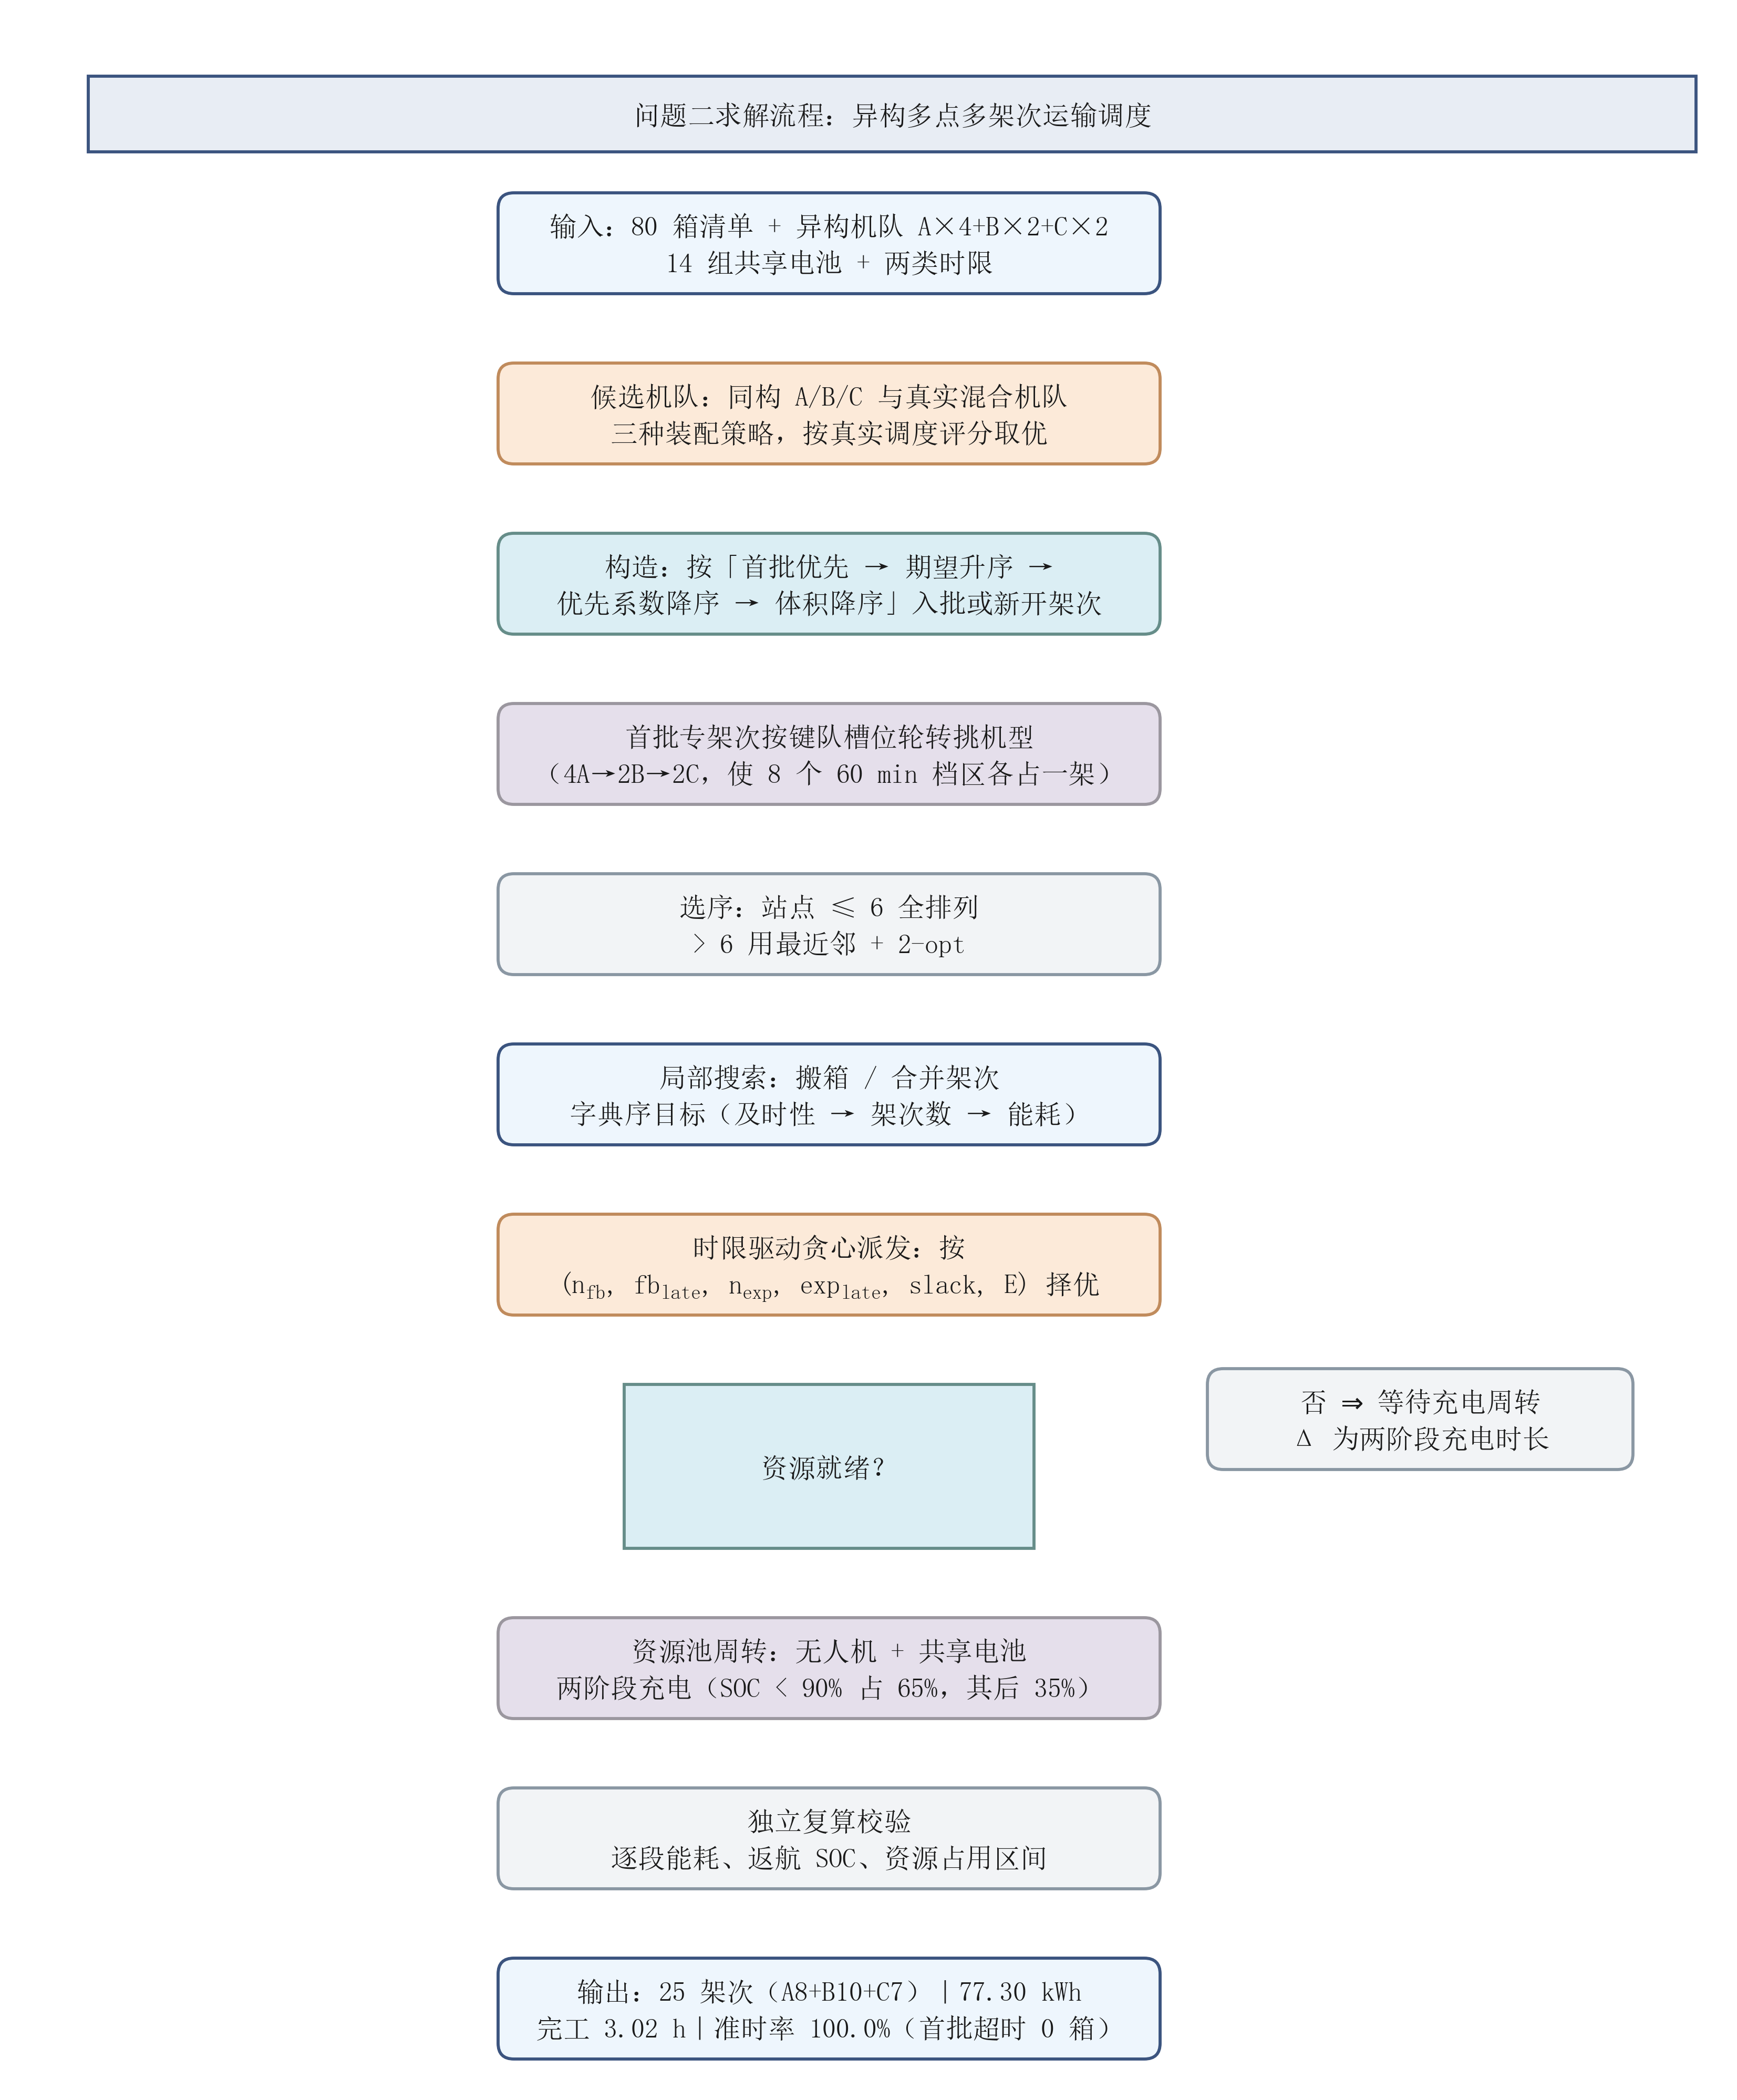
\includegraphics[width=0.86\textwidth]{figures/fig03_flow_q2.png}
	\caption{问题二求解流程}
	\label{fig:flow_q2}
\end{figure}

\textbf{①构造}：货箱按“首批优先 $\rightarrow$ 期望送达升序 $\rightarrow$ 应急优先系数降序 $\rightarrow$ 体积降序”排序，依次尝试并入已有架次或新开架次，并入时校验式~\eqref{eq:21} 的前缀容量约束。其中\textbf{首批箱按机队槽位轮转播种}：$t=0$ 的起始架次不固定选用载重最大的 C 型，而是按 4 架 A 型 $\rightarrow$ 2 架 B 型 $\rightarrow$ 2 架 C 型的顺序让\textbf{每架无人机各认领 1 个 60\,min 档服务区}，从而把高紧迫需求在第一波同时铺开。\textbf{②选序}：站点数 $\le6$ 时枚举全排列，$>6$ 时用最近邻构造再用 2-opt 改进。\textbf{③局部搜索}：以“搬箱、合并架次”为邻域算子，按字典序目标接受改进解。\textbf{④时段驱动贪心派发}：在每个决策时刻，从“资源已就绪”的未调度架次中，选择“新增首批违规最少 $\rightarrow$ 首批迟到量最少 $\rightarrow$ 期望违规最少”者派发；当上述三项指标全部相同时，按\textbf{最小松弛量} $slack=\min_{b}(d_{b}-t_{b}^{deliver})$ 打破平局（\textbf{而非按能耗升序}），即优先放出截止时间最紧的架次。这一设计的动机是：固定顺序调度在资源延迟释放后会失效，而逐时刻按违规量与松弛量择优既能把紧急架次塞进刚刚释放的资源，也不会因为“能耗更低”而把宝贵的首波机位让给非紧迫服务区的第二趟任务——后者正是本节末尾所讨论的两处早期建模缺陷之一。

\textbf{⑤真实调度器复核下的架次合并。}上述四阶段的目标函数用\textbf{乐观代理}估计架次开工时刻，而对外上报的违规由\textbf{真实调度器}判定。两者一旦分叉，优化器就会朝错误方向使劲：把架次权重由 0.05 提高到 0.2 以上，架次数确实能压到 \textbf{25}，但真实排程随即冒出 \textbf{4 箱超期}（准时率降至 \textbf{95.0\%}），而代理目标\textbf{完全看不见}这批违规——把“每违规箱权重” \texttt{violation\_point} 取 $1$ 与取 $10^{3}$ 得到\textbf{逐位相同}的结果，直接证明该目标对真实违规是盲的，即\textbf{“提高架次权重以压架次数”是一个陷阱}。因此本文不靠调参，而是新增 \textbf{\texttt{consolidate\_real} 合并环节}：以“\textbf{真实调度器判定 0 违规}”为\textbf{硬前提}、以“\textbf{架次数最少}”为唯一优化方向，反复尝试 \textbf{①}两两合并架次（容量或能量不可行时\textbf{升级机型}重试）、\textbf{②}按服务区整装重排；\textbf{每个候选方案都必须通过真实调度器复核}，不通过立即回退。同时修掉一处真实缺陷：\texttt{local\_search} 的 \textbf{relocate 走法漏了 \texttt{frozen} 判断}，会把货箱搬出受保护的“首批专架次”（move 2、move 3 均有该判断，只有 move 1 没有）——这正是提高架次权重后首批超时立刻出现的直接原因。修正后架次数由 28 压到 \textbf{25}，而\textbf{违规仍为 0 箱}。

\subsection{计算结果}

\subsubsection{调度方案}

求解得到 \textbf{25 个运输架次}（\textbf{A 型 8 $+$ B 型 10 $+$ C 型 7}，8 架实体无人机\textbf{全部投入使用}）、总运输能耗 \textbf{77.30\,kWh}、全部任务完成时间 \textbf{3.02\,h}（10855.1\,s）、期望送达准时率 \textbf{100.0\%}（\textbf{80/80 箱全部按时送达}，首批违规与期望违规均为 \textbf{0 箱}）。相对本文上一版方案，\textbf{架次数与能耗同时下降}（28 $\to$ 25 个架次、82.30 $\to$ 77.30\,kWh），代价是完工时间由 2.45\,h 延长到 3.02\,h；\textbf{质量装载率由上一版的 71\% 提升到 79\%}（口径为“需求 758\,kg $\div$ 下界 3 轮满载容量 960\,kg”），25 个架次距理论下界 24 个仅高 1 个架次。调度甘特图如图~\ref{fig:q2_gantt} 所示。

\begin{figure}[htbp]
	\centering
	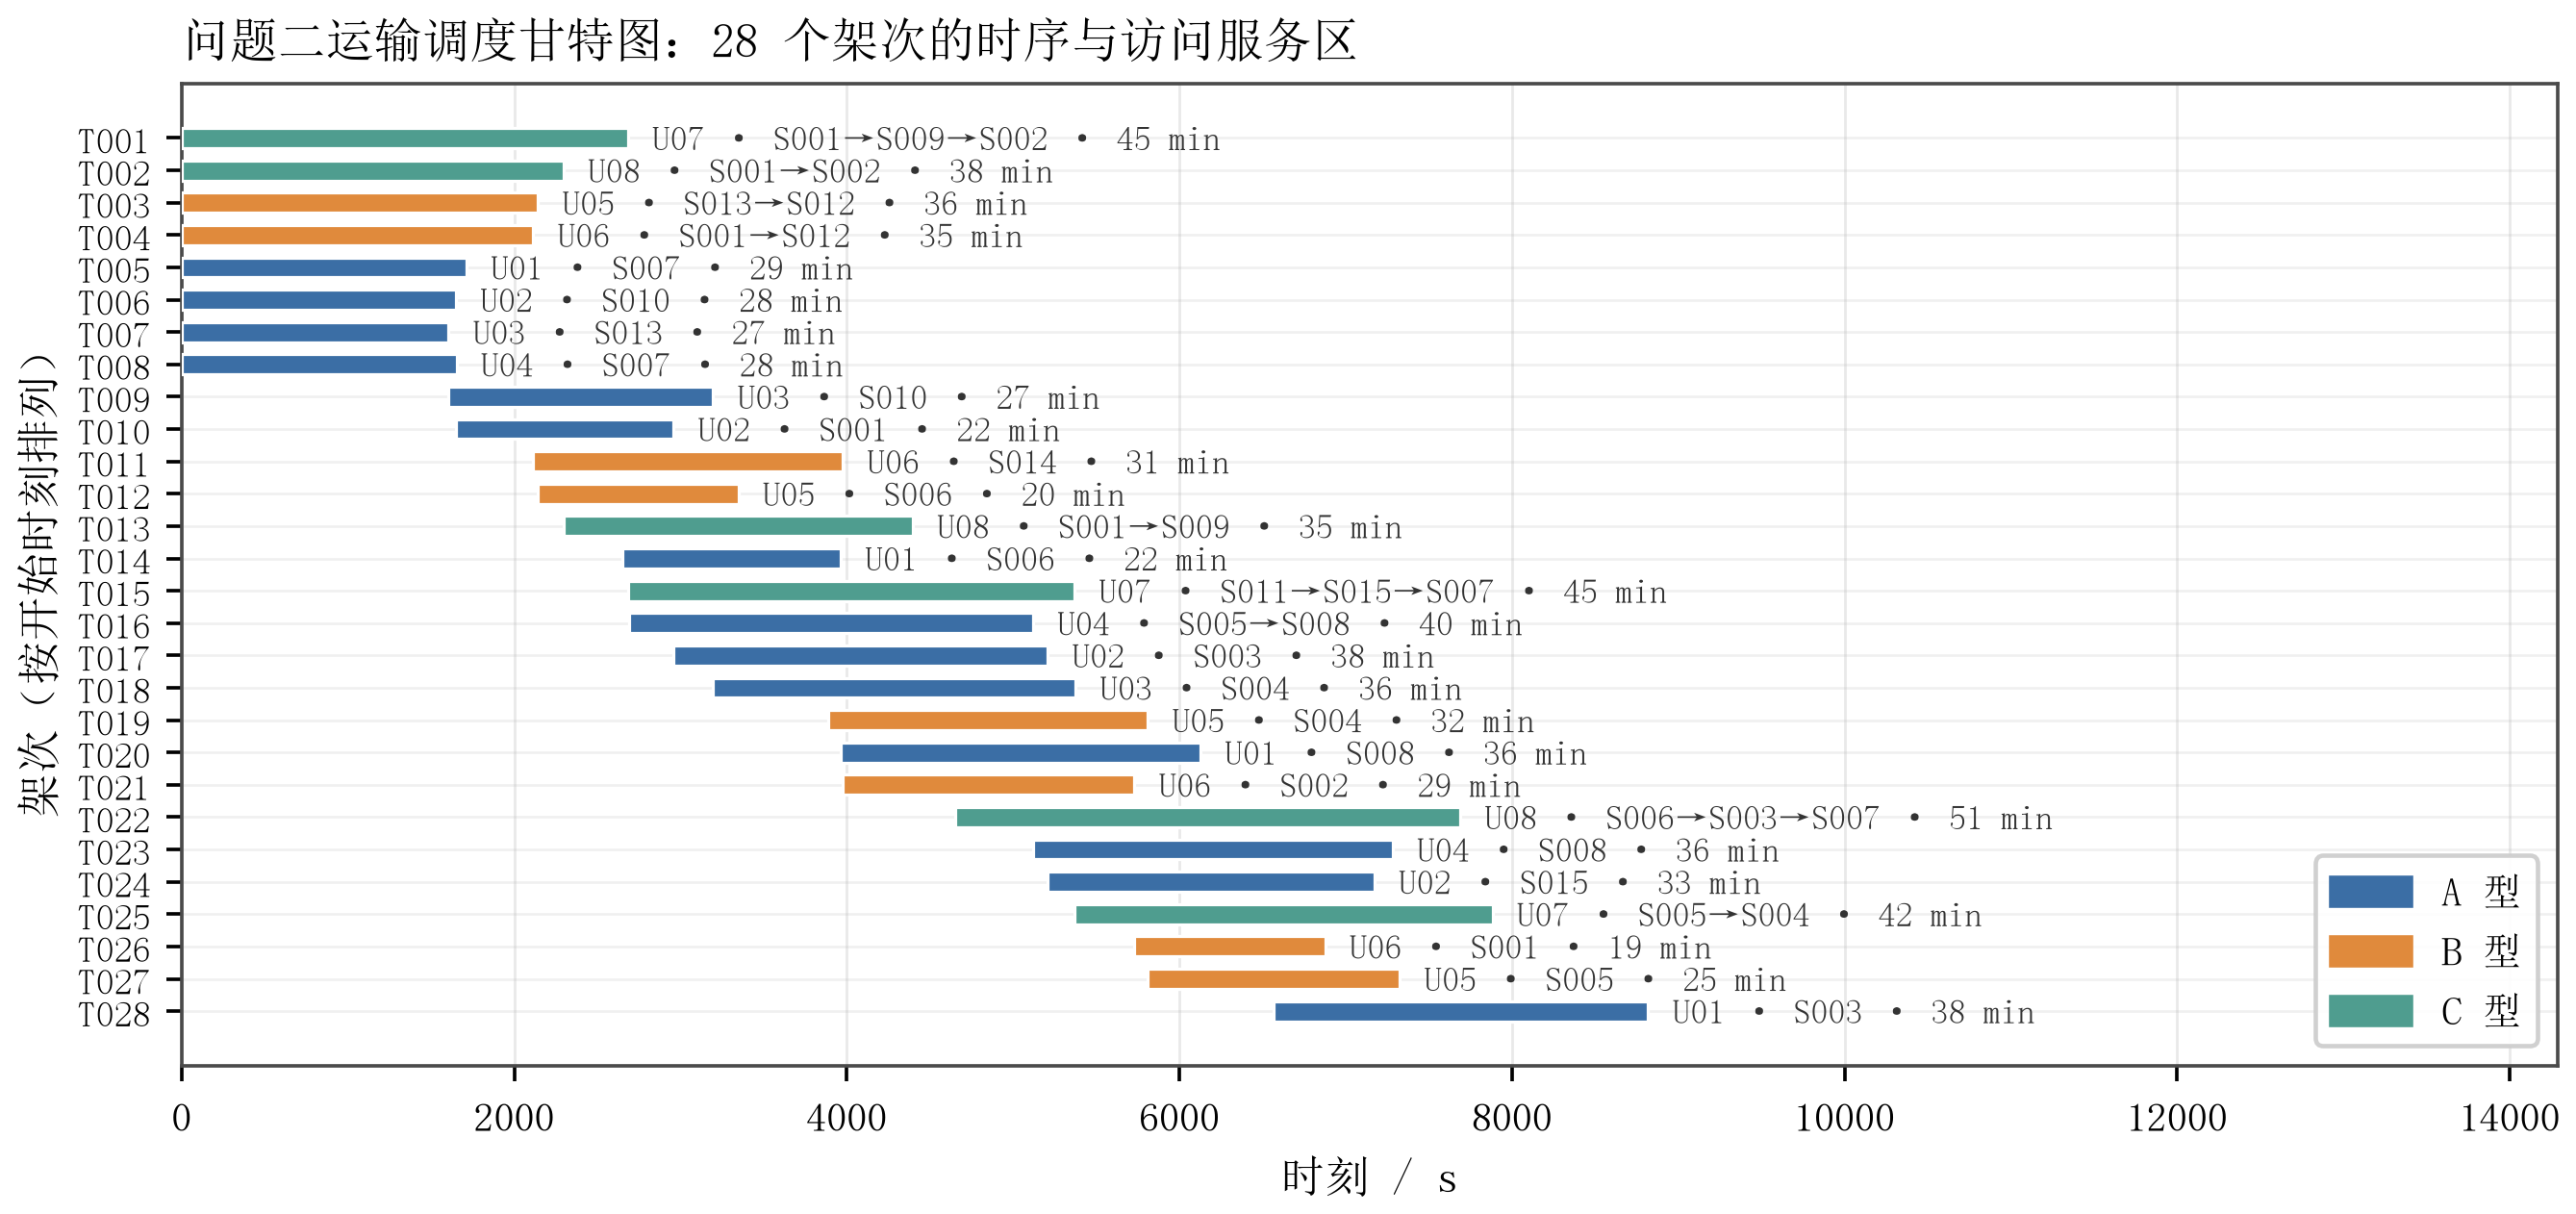
\includegraphics[width=0.98\textwidth]{figures/fig20_q2_gantt.png}
	\caption{运输调度甘特图}
	\label{fig:q2_gantt}
\end{figure}

由图~\ref{fig:q2_gantt} 可见，25 个架次不是“2 条流水线”，而是\textbf{8 架无人机的 8 条并行流水线}：4 架 A 型各执行 2 个架次、2 架 B 型各 5 个、2 架 C 型分别执行 4 个与 3 个，三类机型在时间轴上交错推进，全部任务在 3.02\,h 内完成。这一结果说明\textbf{异构机队必须真正混编使用}，其分工由“容量—航程”互补性自然决定：A 型货舱仅 0.06\,$m^{3}$，单架次只能覆盖 1$\sim$2 个服务区，但其 4.5\,kWh 电池与 25\,km 空载航程恰好适配“单点小批量、距离远”的零散任务（A 型 8 个架次中 6 个为单点架次，单架次能耗仅 1.31$\sim$3.30\,kWh）；B 型居中（5 个单点 $+$ 5 个双点架次）；C 型货舱最大，承担了全部 \textbf{3 个三点架次}（T019、T021、T025）与另外 2 个双点架次，用于承载首批箱密集的大批量串飞。\textbf{若只启用 2 架 C 型机，8 架机队的并行能力将有 3/4 被闲置}——同构 C 型候选方案的完工时间长达 5.32\,h、准时率仅 62.5\%，而采用 8 架混编后分别改善为 3.02\,h 与 100.0\%（见表~\ref{tab:q2_tradeoff}）。图~\ref{fig:q2_payload_decay} 展示了多点架次的载荷递减过程。

\begin{figure}[htbp]
	\centering
	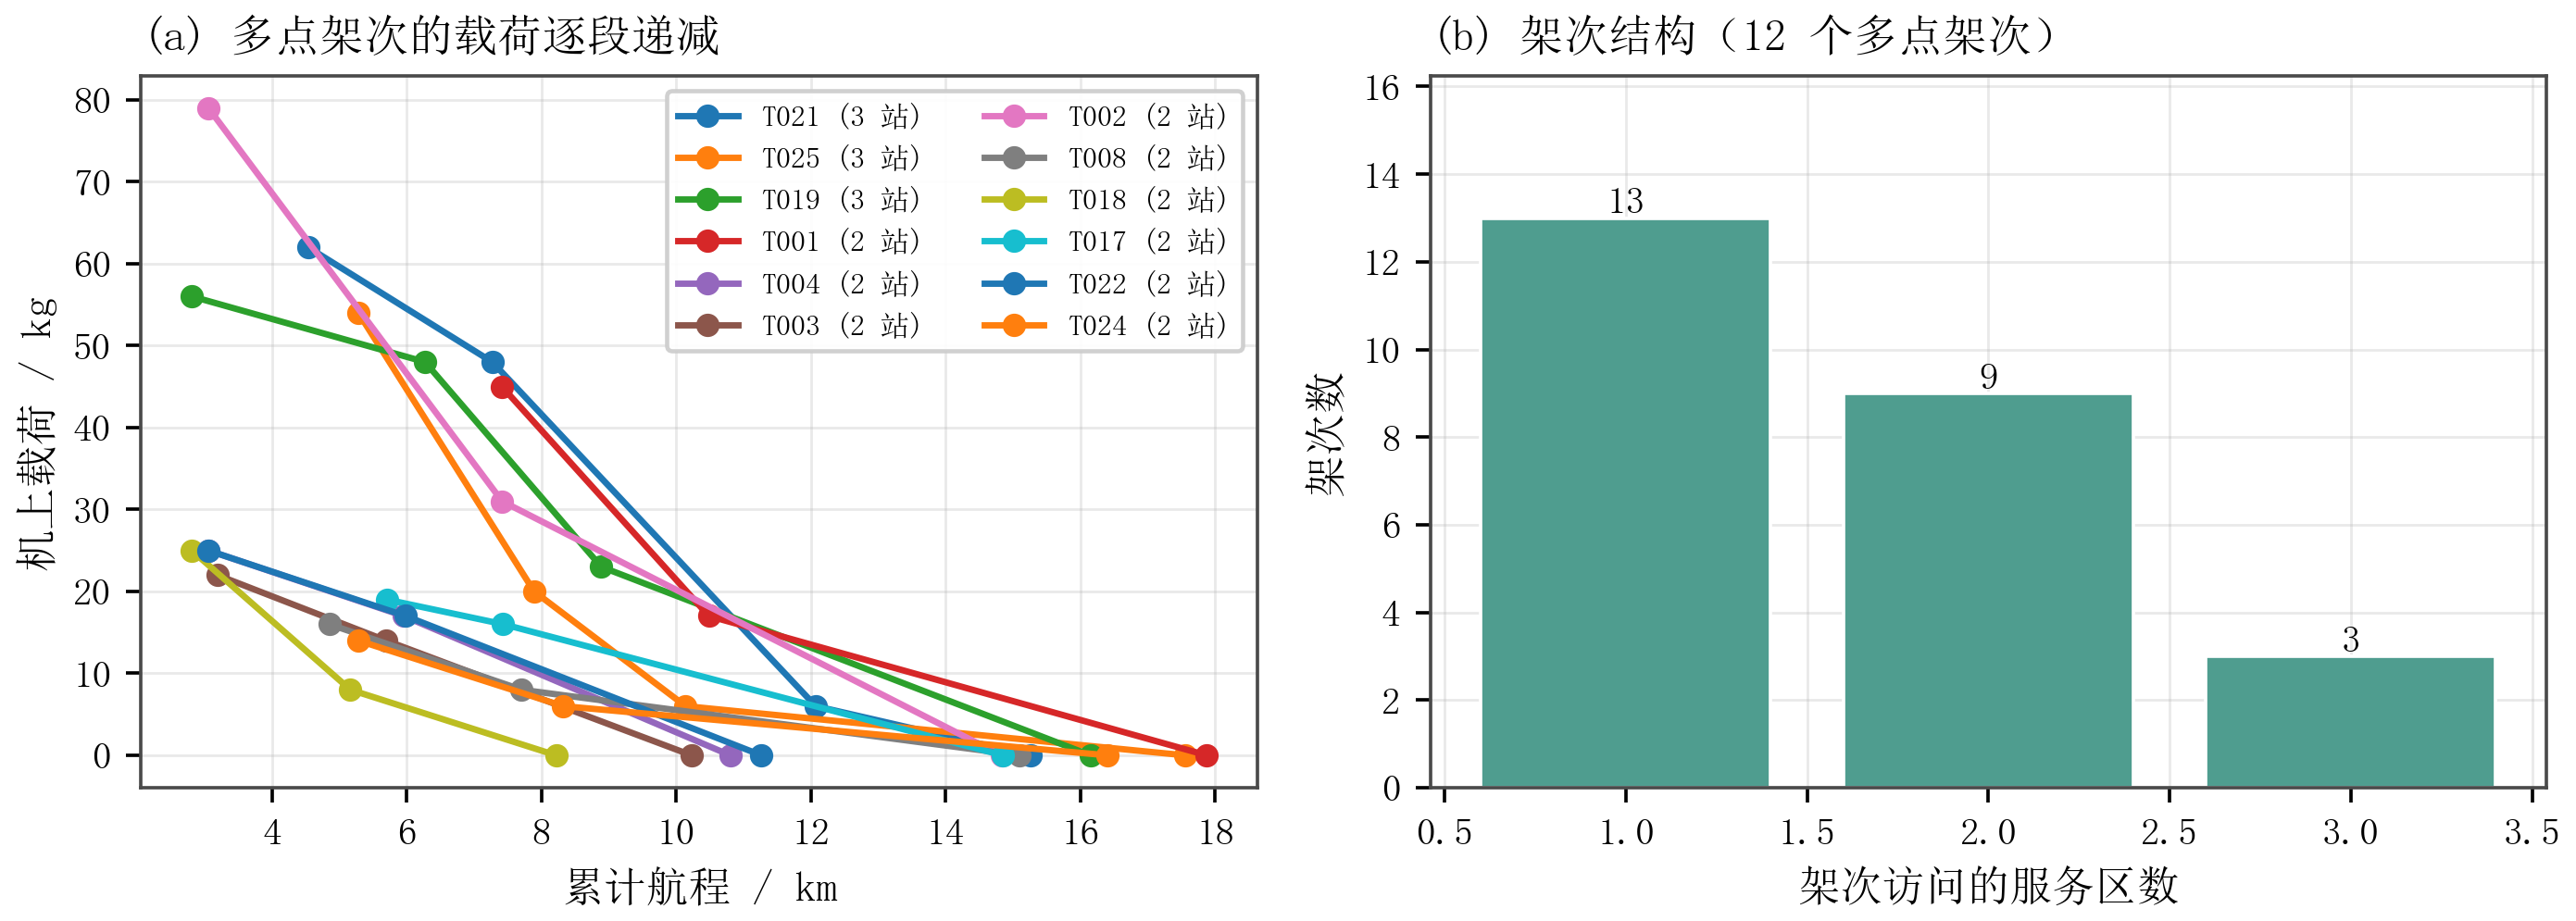
\includegraphics[width=0.98\textwidth]{figures/fig24_q2_payload_decay.png}
	\caption{多点架次的载荷递减与架次结构}
	\label{fig:q2_payload_decay}
\end{figure}

图~\ref{fig:q2_payload_decay}(a) 显示，多点架次的载荷呈阶梯状下降：无人机以最大载荷起飞，每投送一站即卸下该站货物，最后空载返航。这一阶梯特征正是式~\eqref{eq:22} 逐段计算能耗的直观体现——若按“总距离一段”计算，会完全丢失阶梯信息而显著失真。图~\ref{fig:q2_payload_decay}(b) 表明 25 个架次中有 \textbf{12 个为多点架次}（9 个双点、3 个三点，最多 3 站），其余 \textbf{13 个为单点架次}；多点串飞主要由载重与货舱最大的 C 型承担，而 A、B 型以“单点直达”的方式把并行度铺满。这种“少量多点串飞 $+$ 大量单点并行”的组合，正是本问准时率能够达到 100\% 的结构性原因——大批量服务区由 C 型串飞吸收，零散小批量则由 A/B 型并行消化，二者互不挤占资源。

\subsubsection{候选机队与四目标权衡}

为说明“混编 8 架异构机队”的必要性，本文在同一物理口径下比较了 6 种候选机队方案（三种同构机队与三种混合派发规则），结果如表~\ref{tab:q2_tradeoff} 所示；表中“综合得分”即字典序目标的惩罚值（\textbf{越低越好}）。“混合-机队摊平”即本文采用的方案（得分 79.3，为六者最低），其派发规则正是本节的“首批轮转播种 $+$ 最小松弛量打破平局”。\textbf{推荐的正是这一“混合机队 $+$ 机队摊平派发”策略}：只有它在四个目标上同时达到“架次数 25、能耗 77.30\,kWh、准时率 100.0\%、违规 0 箱”，其余候选方案（同构机队或混合但不摊平）要么架次/能耗更差，要么仍留下时限违规。

\begin{table}[htbp]
	\caption{问题二候选机队的四目标对比}
	\label{tab:q2_tradeoff}
	\centering
	\zihao{-5}
	\setlength{\tabcolsep}{4.5pt}
	\begin{tabular}{lccccccc}
		\toprule
		候选机队 & 架次数 & 总能耗/kWh & 完工时间/h & 期望准时率 & 首批违规/箱 & 期望违规/箱 & 综合得分 \\
		\midrule
		同构 C 型 & 14 & 77.94 & 5.32 & 62.5\% & 12 & 30 & 523.2 \\
		同构 B 型 & 33 & 80.50 & 9.56 & 38.8\% & 19 & 49 & 1516.2 \\
		同构 A 型 & 45 & 106.78 & 7.05 & 45.0\% & 15 & 44 & 962.3 \\
		混合-大机型优先 & 28 & 78.98 & 4.88 & 91.2\% & 0 & 7 & 106.2 \\
		混合-小机型优先 & 31 & 83.83 & 5.51 & 82.5\% & 2 & 14 & 173.6 \\
		\textbf{混合-机队摊平} & \textbf{25} & \textbf{77.30} & \textbf{3.02} & \textbf{100.0\%} & \textbf{0} & \textbf{0} & \textbf{79.3} \\
		\bottomrule
	\end{tabular}
\end{table}

由表~\ref{tab:q2_tradeoff} 可见，\textbf{四个目标之间不存在单一最优}：同构 C 型方案的架次数最少（14）、能耗最低（77.94\,kWh），代价是完工时间长达 5.32\,h、准时率只有 62.5\%——它用“少而长”的 C 型串飞换来了能耗最优，却把并行度压缩到 1/4；同构 A 型与 B 型则走向另一个极端，架次数分别膨胀到 45 与 33，能耗与完工时间同时恶化。本文方案与同构 C 型方案相比，架次数多 \textbf{11 个}（25 vs 14），但能耗反而\textbf{略低}（77.30 vs 77.94\,kWh，$-0.8\%$），换回的是\textbf{完工时间下降 43\%}（5.32\,h $\to$ 3.02\,h）与\textbf{期望送达准时率提升 37.5 个百分点}（62.5\% $\to$ 100.0\%）；与本文上一版 28 架次方案相比，则是在\textbf{架次数}（$-10.7\%$）与\textbf{能耗}（$-6.1\%$）上同时改善，仅以完工时间 $+0.57$\,h 为代价。在“及时性 $>$ 架次数 $>$ 能耗”的字典序目标下，这笔交换显然划算；而“混合-大机型优先”与“混合-小机型优先”两个对照方案仍分别留下 7 箱与 14 箱期望违规（见表~\ref{tab:q2_tradeoff}），说明\textbf{混合只是必要条件，“把首波名额在机队槽位上摊平”才是消除违规的充分条件}。

从下界看：单轮机队容量为 \textbf{320\,kg / 0.886\,$m^{3}$}（A$\times$4 $+$ B$\times$2 $+$ C$\times$2 全部满载），而全部需求为 \textbf{758\,kg / 2.011\,$m^{3}$}——按质量需 $758/320=2.37$ 轮、按体积需 $2.011/0.886=2.27$ 轮，取整后至少 3 轮，故\textbf{理论最少架次数为 24}（3 轮 $\times$ 8 架）。本文方案的 \textbf{25 个架次仅比下界多 1 个}（$+4.2\%$）；3 轮满载容量为 $3\times320=960$\,kg / $3\times0.886=2.658$\,$m^{3}$，对应\textbf{质量装载率 $758/960=79\%$、体积装载率 $2.011/2.658=76\%$}（上一版 28 架次时为 71\%）。需要说明的是，这一压缩\textbf{并非来自放宽自加的限制}：把单架次\textbf{站数上限}由 3 放宽到 4、5、6，结果\textbf{完全不变}，说明站数上限并非紧约束；真正造成碎片化的是 \textbf{A 型货舱 0.06\,$m^{3}$ 仅装得下约 2 箱}的体积瓶颈。这也说明“混编 8 机”在架次数维度上已接近极限。

\subsubsection{资源使用与充电周转}

无人机与共享电池的占用情况如图~\ref{fig:q2_resources} 所示。

\begin{figure}[htbp]
	\centering
	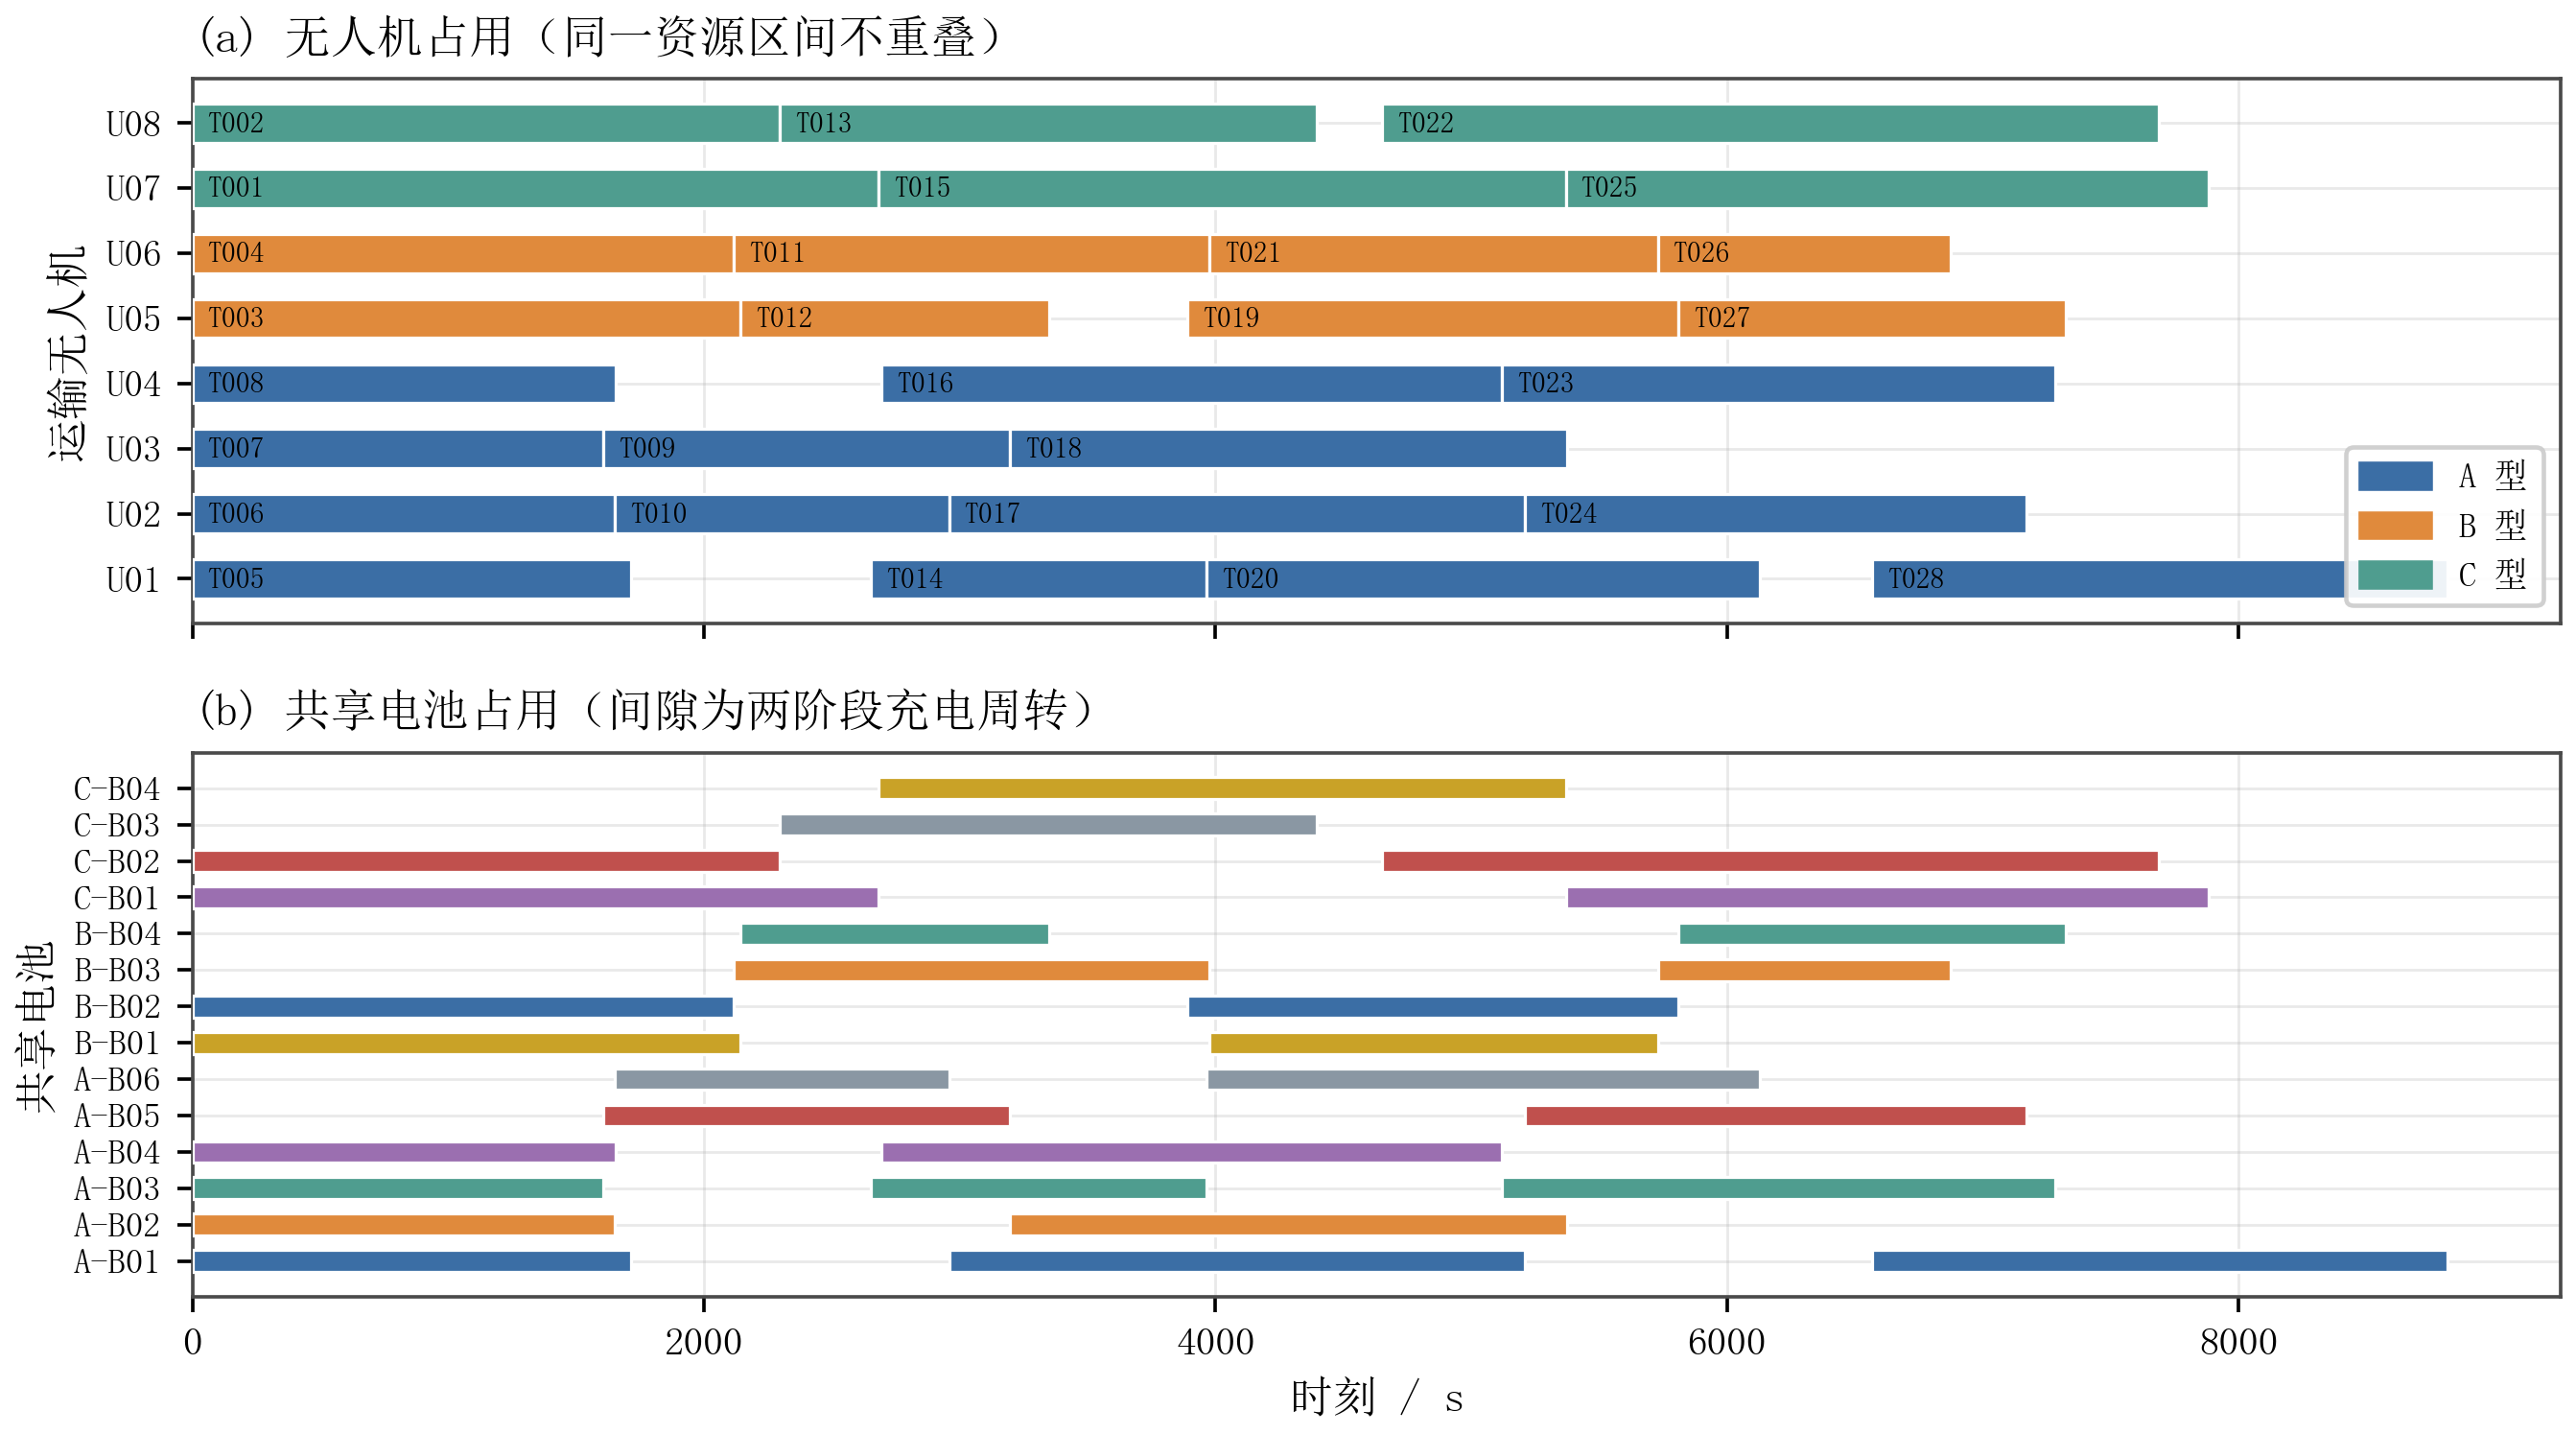
\includegraphics[width=0.98\textwidth]{figures/fig21_q2_resources.png}
	\caption{无人机与共享电池的占用时序}
	\label{fig:q2_resources}
\end{figure}

图~\ref{fig:q2_resources}(a) 显示 8 架运输无人机 U01$\sim$U08 各自的架次区间\textbf{互不重叠}——即无人机刚返回 O01 即可接续下一个架次，这正是资源利用率最大化的表现：8 架无人机的累计飞行时长为 \textbf{3490.2$\sim$9833.4\,s}（占完工时间 \textbf{32.2\%$\sim$90.6\%}），其中 U02 与 U03 的两个架次首尾严格相接（$0\to1713.5\to3876.3$\,s 与 $0\to1311.1\to3490.2$\,s），实现\textbf{零空闲}；U07 承担 4 个架次、累计飞行 \textbf{9833.4\,s}（占完工时间 \textbf{90.6\%}），为全队最高。图~\ref{fig:q2_resources}(b) 中电池条之间的空白即为\textbf{两阶段充电周转}窗口：A/B/C 型电池的等效满充时间分别为 30/40/50\,min，而单架次时长介于 \textbf{20$\sim$51\,min}，二者量级相当，因此\textbf{电池周转与无人机占用共同决定完工时间}——14 组共享电池的周转次数分别为 A 型 1、2、2、1、1、1，B 型 3、3、2、2，C 型 2、2、2、1，各组负载均衡，没有哪一组电池成为瓶颈。

\subsubsection{时限达成情况}

逐箱的时限达成情况如图~\ref{fig:q2_timeliness} 与图~\ref{fig:q2_lateness} 所示。

\begin{figure}[htbp]
	\centering
	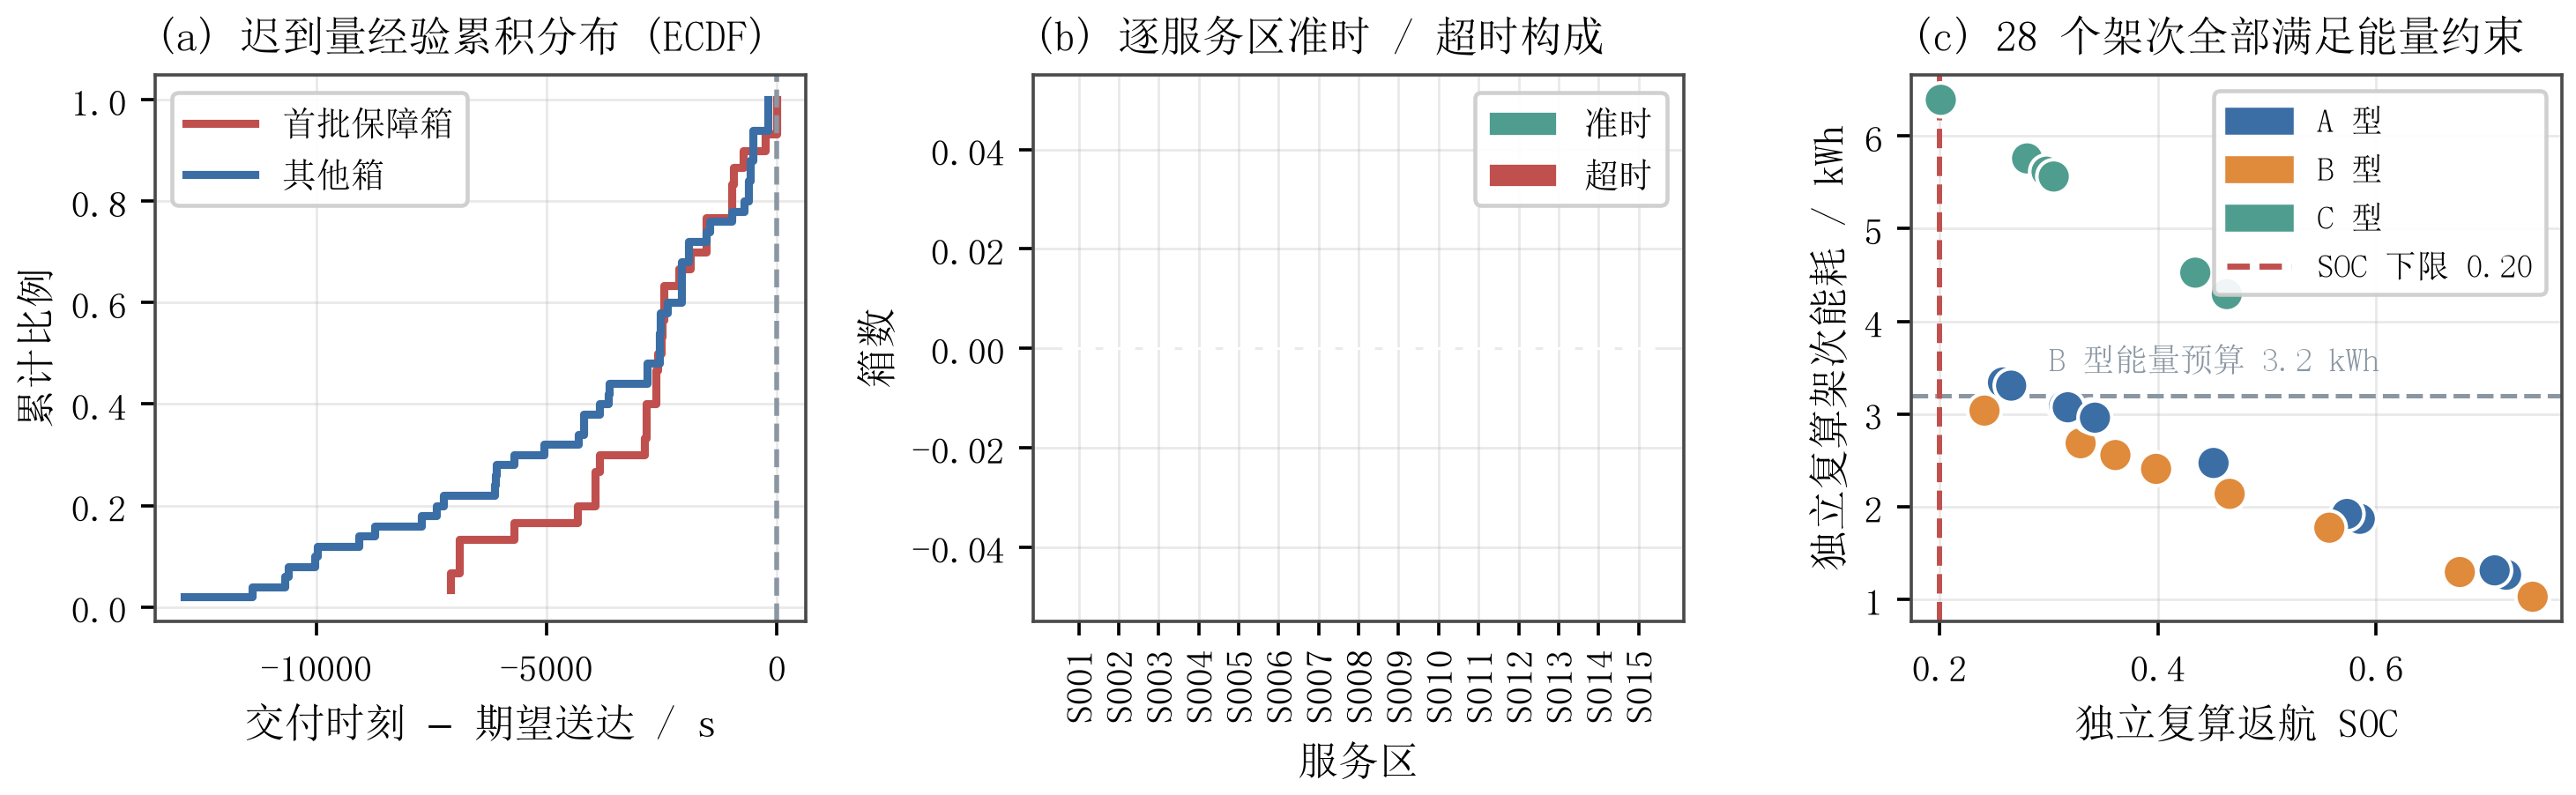
\includegraphics[width=0.98\textwidth]{figures/fig22_q2_timeliness.png}
	\caption{物资时限达成分析}
	\label{fig:q2_timeliness}
\end{figure}

\begin{figure}[htbp]
	\centering
	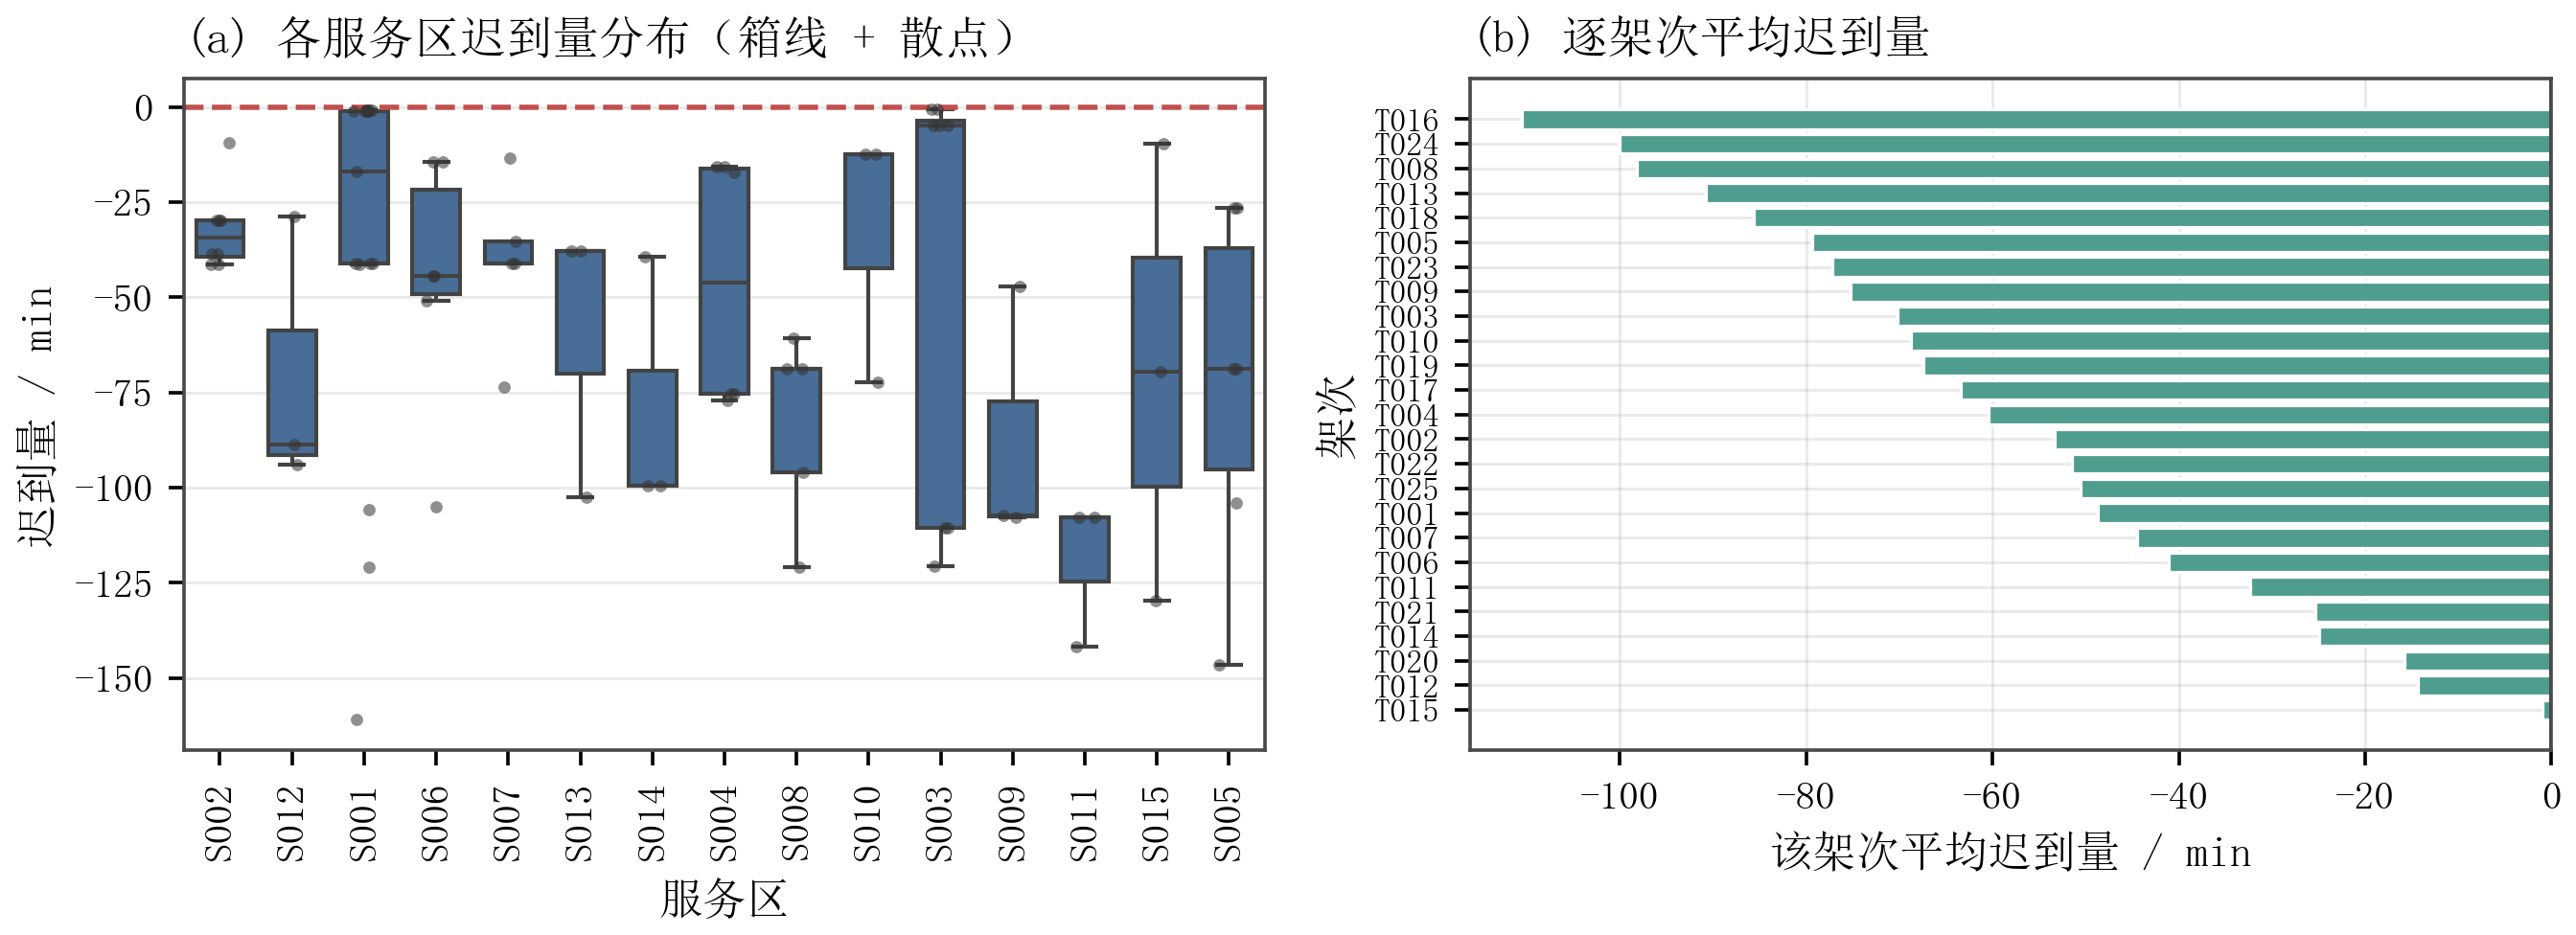
\includegraphics[width=0.98\textwidth]{figures/fig25_q2_lateness.png}
	\caption{迟到量分布}
	\label{fig:q2_lateness}
\end{figure}

由图~\ref{fig:q2_timeliness}(a) 的 ECDF 可见，全部 \textbf{80 箱的交付时刻均早于各自的期望送达时间}——曲线在 0 处收敛于 1.0，\textbf{准时率 100.0\%}、最大迟到量 \textbf{0\,s}；30 个首批保障箱也全部在首批截止时间前送达。图~\ref{fig:q2_timeliness}(b) 的逐服务区构成显示 S001$\sim$S015 \textbf{全部服务区均无超时箱}。图~\ref{fig:q2_lateness}(a) 进一步显示各服务区的“迟到量”全部为负值（即提前量）：最紧的 S003、S010、S001 提前量中位数约 5$\sim$17\,min，最宽松的 S009、S011 提前量中位数约 1.8\,h；全部 80 箱中最大提前量为 \textbf{2.68\,h}（S001-HYG-01），最小仅 \textbf{35.5\,s}（S003-MED-01，截止 7200\,s）；图~\ref{fig:q2_lateness}(b) 的逐架次平均提前量同样全部落在 0 的左侧，说明时限裕度分布在全部 25 个架次上，而非集中在个别架次。

\subsection{方案可行性检验与独立复算}

按独立校验的要求，本文对 25 个架次做了两条并行的检验路径。

\textbf{（1）独立校验器的判定。}校验器从附件参数与 DEM 出发、不引用求解器的任何中间结果，重算全部物理量并逐条比对。其报告 \textbf{0 条违规}：\textbf{能量、SOC、时间自洽、资源占用、通信五类物理硬约束的违规均为 0 条}，且\textbf{首批超时与期望超时两类时限约束同样为 0 条}（80 箱全部按时送达），说明方案在物理与时限两个层面上均已可行。

\textbf{（2）基于航段缓存的独立复算。}为交叉验证，本文另用 240 条完整航段缓存对全部 25 个架次做了\textbf{逐段独立重算}：按式~\eqref{eq:4} 计算每段等效航程、按式~\eqref{eq:5} 计算能耗、按载荷递减规则确定每段机上载荷，结果如图~\ref{fig:q2_audit} 所示。

\begin{figure}[htbp]
	\centering
	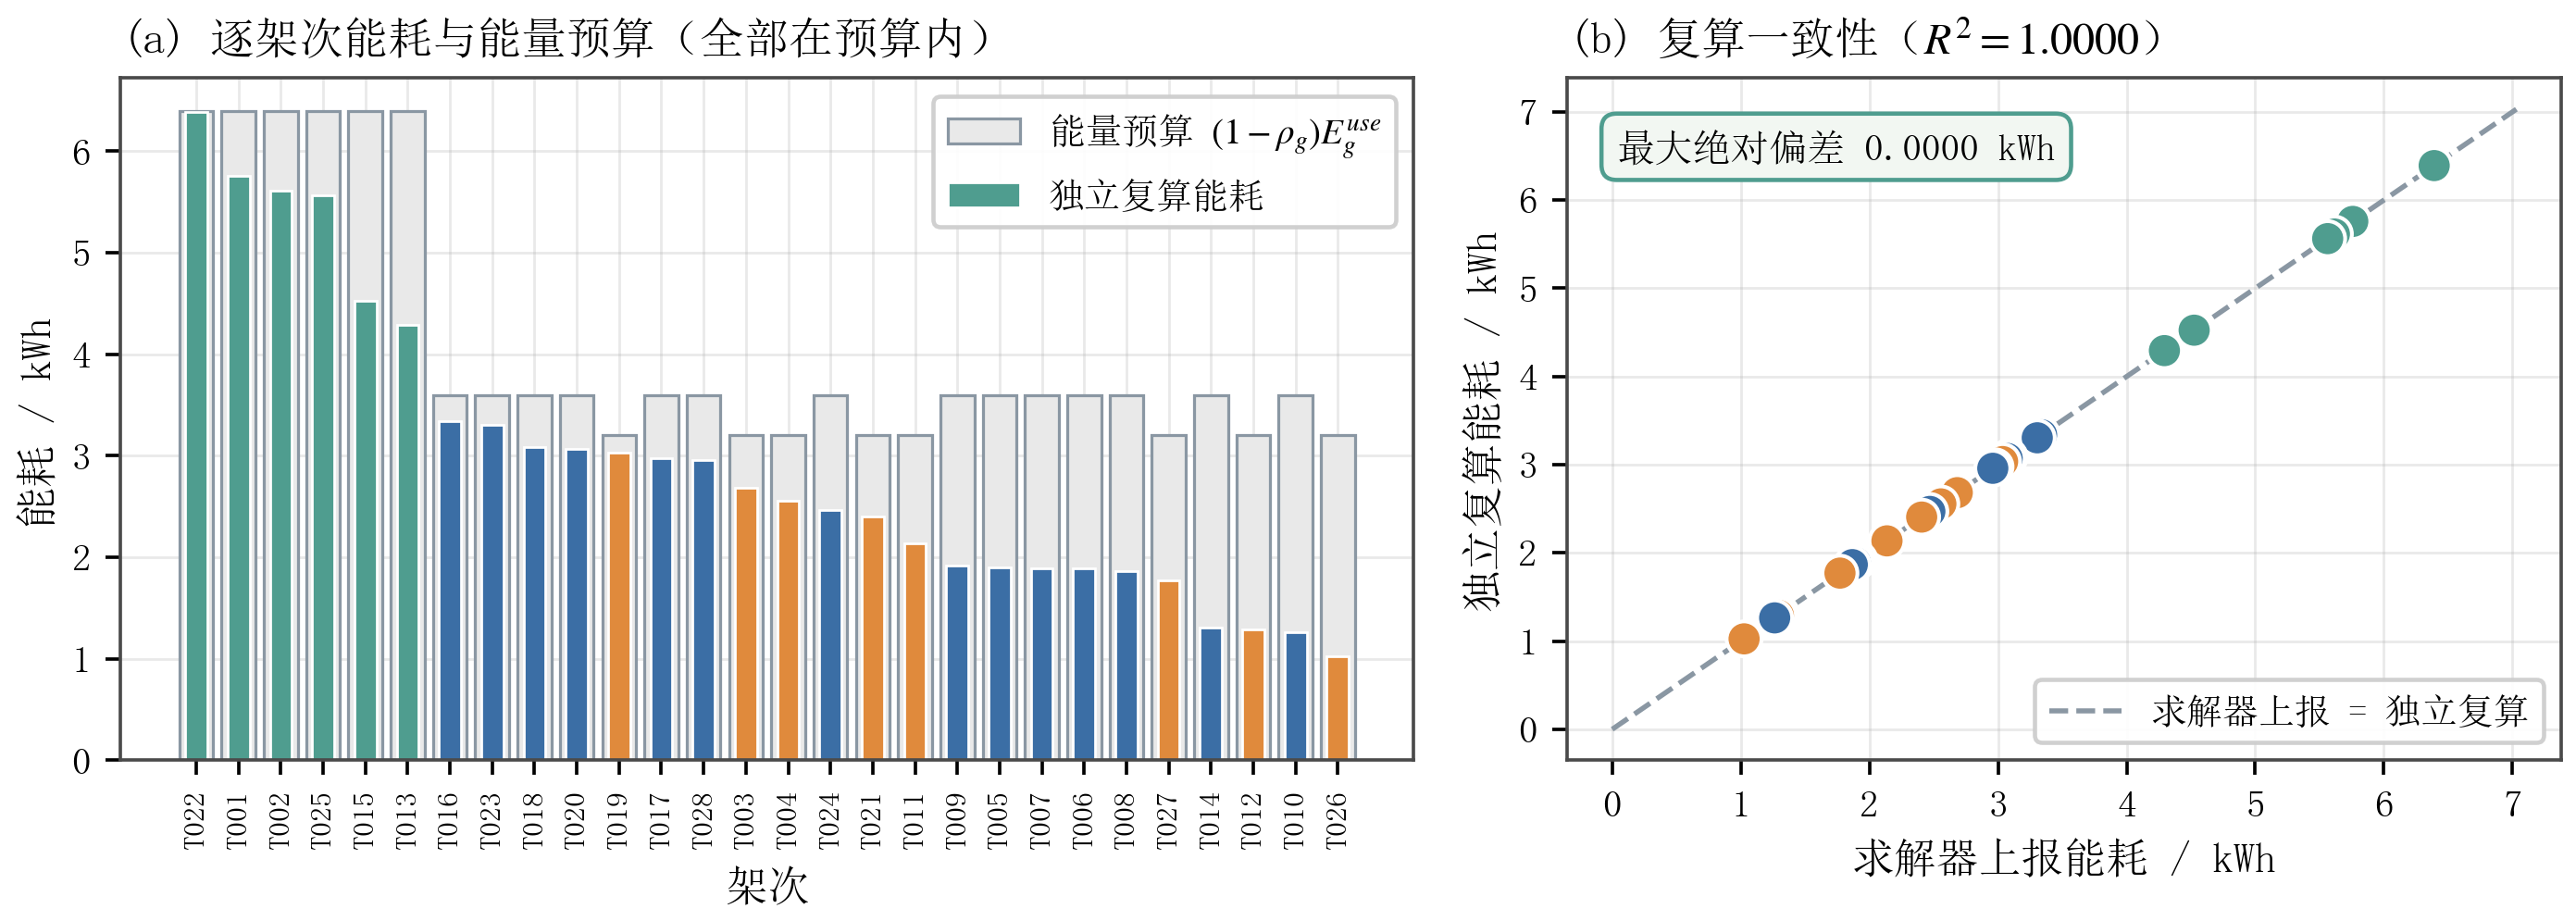
\includegraphics[width=0.98\textwidth]{figures/fig23_q2_energy_audit.png}
	\caption{逐架次能耗与能量预算对比}
	\label{fig:q2_audit}
\end{figure}

图~\ref{fig:q2_audit}(a) 表明\textbf{25 个架次的独立复算能耗全部落在各自的能量预算之内}（A/B/C 型的可用能量分别为 $3.6/3.2/6.4$\,kWh，逐架次实际消耗 1.29$\sim$6.40\,kWh）；图~\ref{fig:q2_audit}(b) 以散点形式给出两套计算的逐架次对照。两套计算的总能耗均为 \textbf{77.3016\,kWh}，与求解器上报值一致。此外，独立复算得到的架次结束时刻与“开始 $+$ 准备 $+$ 装载 $+$ 飞行 $+$ 逐站交接”的\textbf{自洽偏差最大 0.078\,s}（远小于 0.1\,s）、按方案自报区间检查的\textbf{资源占用冲突为 0}。

两条独立路径得出\textbf{一致结论}：方案在能量、时间、资源与时限四个维度上均可行，\textbf{违规总数为 0 条}。图~\ref{fig:q2_audit_detail} 汇总了全部七类校验项的违规分布。

\begin{figure}[htbp]
	\centering
	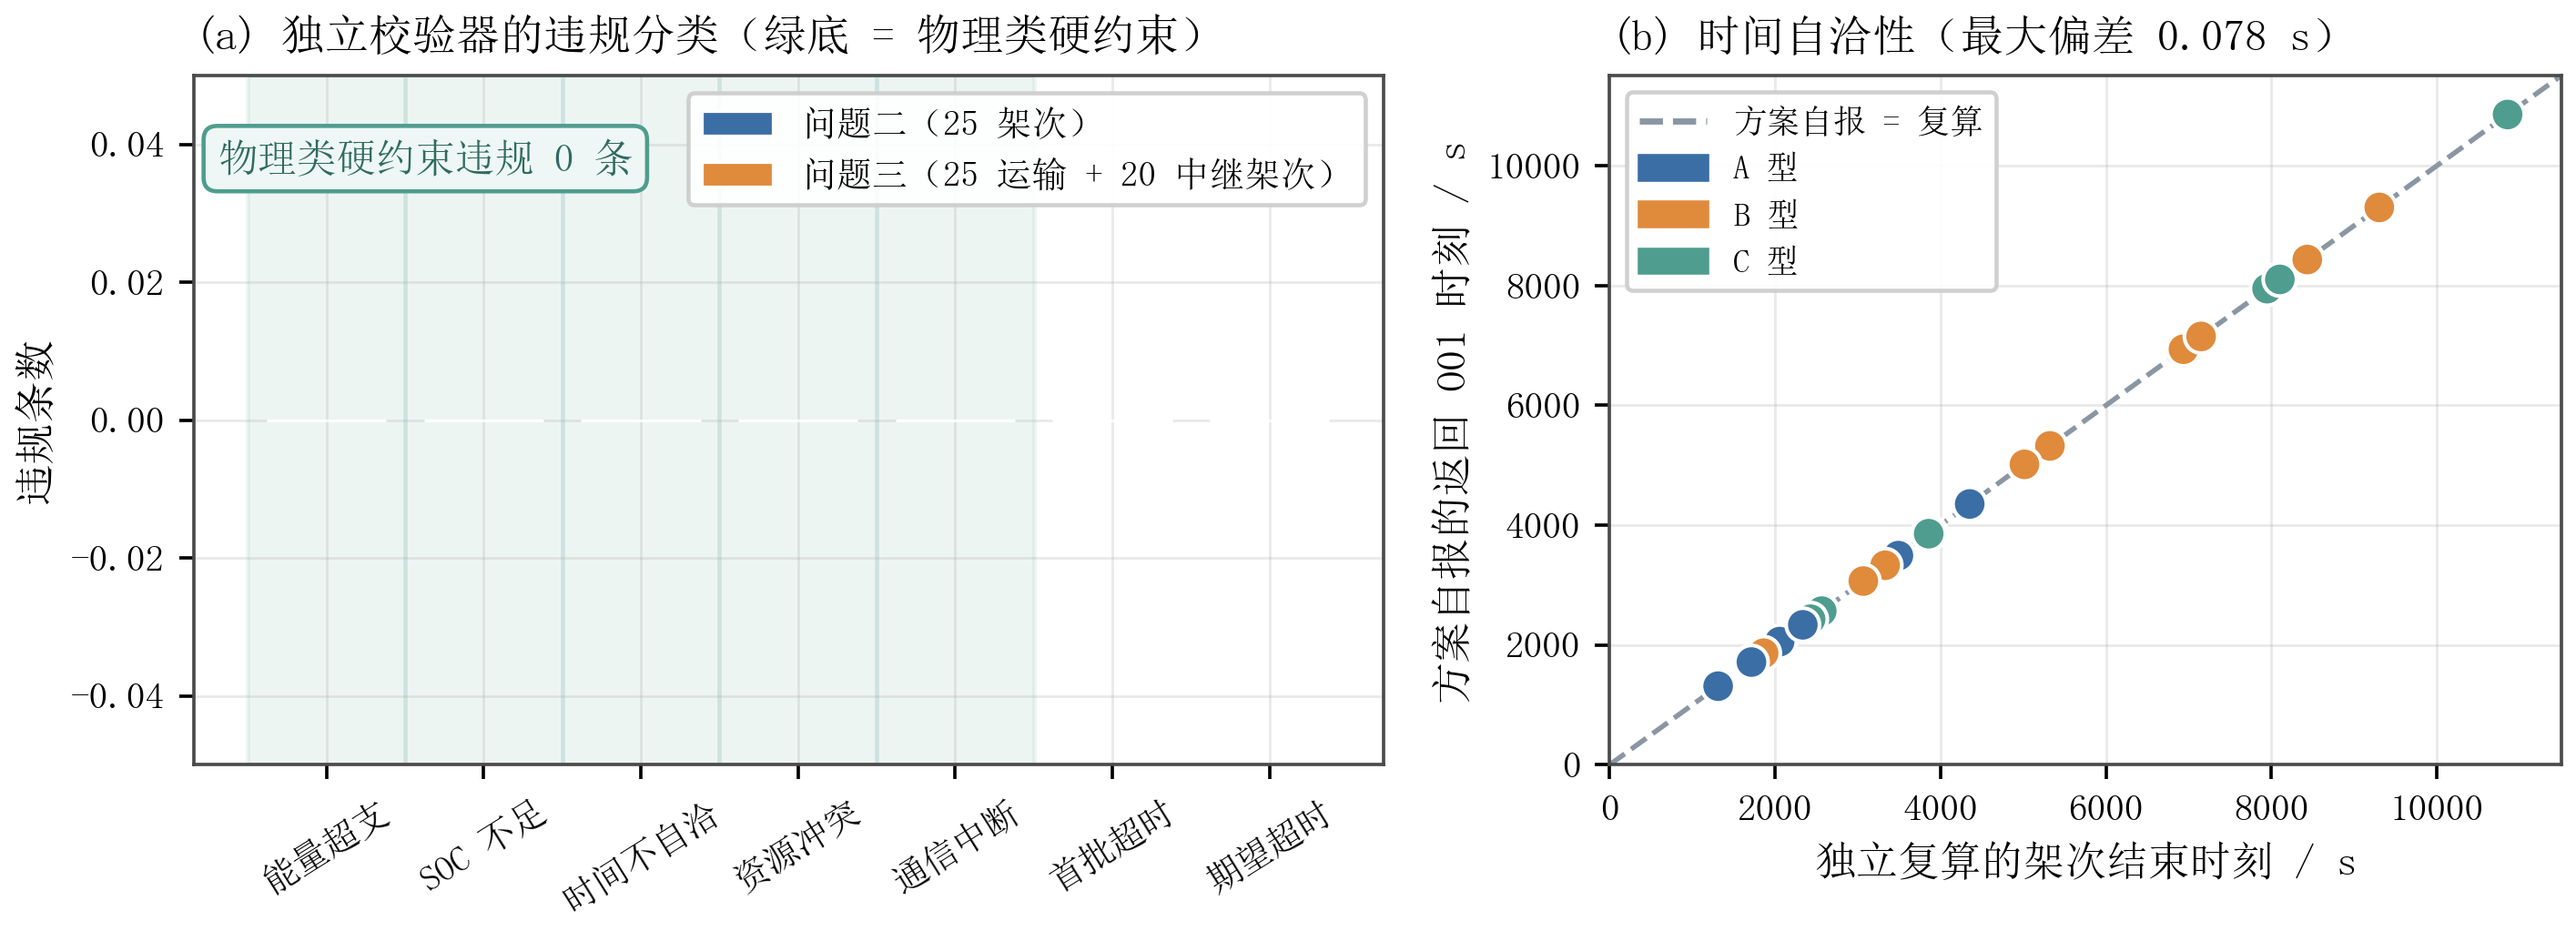
\includegraphics[width=0.98\textwidth]{figures/fig37_q2_audit.png}
	\caption{独立校验结果汇总}
	\label{fig:q2_audit_detail}
\end{figure}

由图~\ref{fig:q2_audit_detail}(a) 可见，在能量超支、SOC 不足、时间不自洽、资源冲突、通信中断这五类\textbf{物理硬约束}以及首批超时、期望超时这两类时限约束上，问题二与问题三的违规数\textbf{全部为 0}（图中绿底区域，图例同时给出两问的架次数）；图~\ref{fig:q2_audit_detail}(b) 以散点形式给出时间自洽性检验，所有点均落在对角线上，最大偏差 0.078\,s。

\subsection{首批保障时限的可行性：一次误判的纠正}

本问最关键的结论是：\textbf{首批保障时限在本机队下是可行的}——8 个 60\,min 档服务区全部按时送达。由于本文早期版本的求解器曾得出相反结论，此处如实记录误判的定位与纠正过程。

\textbf{第一步，供给与需求的数量对偶。}供给侧是异构机队 \textbf{A$\times$4 $+$ B$\times$2 $+$ C$\times$2 $=$ 8 架}运输无人机；需求侧首批截止为 60\,min 的服务区恰为 \textbf{8 个}（S001、S002、S006、S007、S010、S012、S013、S014），每区 2 个首批箱共 16 箱。单架次能力并不构成瓶颈：每个服务区的首批箱合计仅 17\,kg / 0.039\,$m^{3}$，实测最早的 60\,min 档投送在 \textbf{934.3\,s}（S006）即已完成，远早于 3600\,s。因此只要在 $t=0$ 为\textbf{每架无人机各派 1 个架次}、并让这 8 个起始架次分别覆盖 8 个高紧迫服务区，第一小时的\textbf{供给架次数（8）恰好等于需求架次数（8）}，首批时限\textbf{恰好可行}——这也解释了为何 60\,min 档最晚的一箱（S001）交付于 \textbf{3546.3\,s}、裕度仅 \textbf{53.7\,s}：方案正是贴着该对偶的临界点构造出来的。

\textbf{第二步，早期误判的两个建模缺陷。}早期版本之所以得到“首批保障时限物理不可行、任何调度算法都无法消除”的结论，根源是两处\textbf{建模缺陷}，而非资源不足：

\begin{itemize}[leftmargin=2em]
	\item \textbf{（a）机队坍缩。}候选机队只评估了三种\textbf{同构}机队（全 A / 全 B / 全 C），把 8 架异构机队实际压缩成“仅 2 架 C 型机”在用，等于\textbf{闲置了 3/4 的并行能力}。由此推出的“第一个小时内至多完成 2 个架次”看似是一个严格的供给上界，实际上只是机型选择造成的假象。
	\item \textbf{（b）派发规则退化。}派发器在尚无线限违规时按\textbf{能耗升序}打破平局，于是首波 8 个名额中有 2 个被第二趟 S001 架次占用，而若干 60\,min 档服务区的首批箱被推迟到远超 3600\,s 的时刻。由于三个时限档的实际裕度本就只有几十秒量级（见第三步），这种“把首波机位让给能耗更低任务”的排序足以制造出大批首批超时。
\end{itemize}

两处缺陷叠加，才产生了早期版本所报告的“首批超时 17 箱、期望超时 19 箱”的假象。换言之，\textbf{“物理不可行”并非资源的必然结果，而是“机队坍缩 $+$ 派发退化”的产物}。

\textbf{第三步，修正与结果。}修正对应三点：其一，机队评估改为 \texttt{auto} 模式，在三种同构机队之外\textbf{同时评估真实的混合机队}（A$\times$4 $+$ B$\times$2 $+$ C$\times$2）；其二，首批播种架次在机队槽位上\textbf{轮转}（4 架 A $\to$ 2 架 B $\to$ 2 架 C），且派发平局按\textbf{最小松弛量} $slack=\min_{b}(d_{b}-t_{b}^{deliver})$ 决出而非按能耗；其三，\texttt{local\_search} 的 relocate 走法补上 \texttt{frozen} 判断（此前它会把货箱搬出受保护的首批专架次），并以\textbf{真实调度器}对每个候选方案逐条复核（见求解算法第 \textbf{⑤} 点）。修正后三类时限档的实测表现（对应表~\ref{tab:q2_tradeoff} 中的“混合-机队摊平”方案）为：\textbf{60\,min 档 8 个服务区全部在 3600\,s 内交付}（最晚 S001 为 3546.3\,s）、\textbf{120\,min 档最晚 7164.5\,s}（S003，裕度仅 35.5\,s）、\textbf{180\,min 档最晚 7966.6\,s}（S009），\textbf{首批违规 0 箱、期望违规 0 箱}，期望送达准时率 \textbf{100.0\%}（80/80 箱）；独立校验器对全部校验项报出 \textbf{0 条违规}。

这一纠正过程本身具有方法论意义：\textbf{在应急调度中，把异构机队先入为主地简化成单一机型，会系统性地低估并行能力，并进而把“建模缺陷”误判为“物理不可行”}——而“不可行”这类否定性结论必须先用“供给 $=$ 需求”的数量对偶检验，再考虑是否需要放宽口径。
